\section{Созданиe программы wave\_find\_path c использованием sc-памяти}
\label{Desc_libscprg}

В этом разделе мы будем создавать программу поиска минимального пути с
использованием библиотеки \verb|libsc|. По примененному алгоритму
поиска минимального пути и своей структуре программа из этого раздела
будет похожа на программу из раздела~\ref{Desc_prg}. Самым важным
отличием будет то, что обработка информации происходит в sc-памяти.

Начнем мы с подготовки sc-памяти для работы алгоритма.

\subsection{Инициализация и подготовка sc-памяти}
\label{libscprg_init_sc_memory}

Создадим набросок функции \lstinline|main| для начала работы с
sc-памятью:
\begin{lstlisting}[texcl]
// Необходимые заголовычные файлы
#include <libsc.h>
#include <pm_keynodes.h>

// $\dots$

int main(int argc, char **argv)
{
    // 1. Инициализация libsc.
    sc_session *system = libsc_init();

    // Теперь мы получили пустую sc-память.

    // 2. Создание sc-сегмента \verb|/proc/keynode| и
    // системных ключевых узлов в нем (например, \verb|1_|, \verb|2_| и т.д.)
    // Эту функцию нужно вызывать обязательно.
    pm_keynodes_init(system);

    // \dots

    // 7. Закроем пользовательскую сессию.
    session->close();

    // 8. Деинициализируем libsc.
    libsc_deinit();

    return 0;
}
\end{lstlisting}

Я думаю, что комментарии к приведенному выше листингу излишне. Если же
у вас возникли трудности, то обратитесь к
разделу~\ref{Begin_with_libsc}, в котором были описаны все
использованные функции.

Мы получили sc-память с системными ключевыми узлами, однако для работы
алгоритма необходимы еще и такие ключевые узлы, как
\idtf{неориентированный граф}, \idtf{вершина\_}, \idtf{ребро\_} и др.,
т.е. ключевые узлы базы знаний по теории графов
(см. раздел~\ref{sec:Onto_concept_list}). Однако, по данному
пункту есть два отличия от раздела~\ref{sec:Onto_concept_list}.

Во-первых, реализация sc-памяти имеет сегментную организацию, поэтому
необходимо выбрать сегмент, в котором будут храниться ключевые узлы
базы знаний по теории графов. Для этого мы бдуем использовать сегмент
\verb|/graphs_theory/keynode|.

Во-вторых, реализация sc-памяти работает только с кодировкой
\verb|CP1251|, а исходники примера подготовлены в кодировке
\verb|UTF-8|, поэтому при решении нашей задачи не очень удобно
использовать русские идентификаторы ключевых узлов. Таким образом, мы
будем использовать в исходном тексте английские идентификаторы
ключевых узлов, например:
\begin{itemize}
\item \idtf{вершина\_} $\Leftrightarrow$ \idtf{vertex\_}
\item \idtf{связка\_} $\Leftrightarrow$ \idtf{connective\_}
\item \idtf{ребро\_} $\Leftrightarrow$ \idtf{edge\_}
\item \idtf{дуга\_} $\Leftrightarrow$ \idtf{arc\_}
\item \idtf{неориентированный граф} $\Leftrightarrow$ \idtf{undirected graph}
\item \idtf{ориентированный граф} $\Leftrightarrow$ \idtf{directed graph}
\item \idtf{простая цепь*} $\Leftrightarrow$ \idtf{simple trail*}
\end{itemize}

Теперь можно переходить к организации создания и работы с ключевыми
узлами. Для этого нам понадобится функция создания сегмента по полному
\verb|URI|, которая определена в файле \verb|segment_utils.h|
следующим образом:
\begin{lstlisting}[texcl]
/// Функция при помощи sc-сессии @p s создает sc-сегмент по полному URI @p uri
/// c созданием всех промежуточных директорий.
///
/// Если создание прошло успешно, то sc-сегмент, иначе 0.
sc_segment *create_segment_full_path(sc_session *s, const sc_string &uri);
\end{lstlisting}

Напишем код, который обеспечивает работу с ключевыми
узлами. В листинге ниже представлено пространство имен
\lstinline|graph_theory|, которое содержит объявление ключевых узлов и
функцию для их инициализации:
\begin{lstlisting}[texcl]
// Для использования \verb|create_segment_full_path|
#include <segment_utils.h>

// $\dots$

/// Пространство имен ключевых узлов по теории графов.
///
/// Для начала работы необходимо вызвать функцию \verb|graph_theory::init|,
/// передав в качестве параметра системную сессию.
/// После этого, например, чтобы обратиться к узлу \idtfm{вершина\_},
/// достаточно написать \verb|graph_keynodes::vertex_|.
namespace graph_theory
{
    /// URI сегмента ключевых узлов.
    const char *segment_uri = "/graph_theory/keynode";

    /// Созданный сегмент ключевых узлов.
    sc_segment *segment;

    /// Массив идентификаторов ключевых узлов.
    const char *idtfs[] = {
        "vertex_",          // \idtfm{вершина\_}
        "connective_",      // \idtfm{связка\_}
        "edge_",            // \idtfm{ребро\_}
        "arc_",             // \idtfm{дуга\_}
        "undirected graph", // \idtfm{неориентированный граф}
        "directed graph",   // \idtfm{ориентированный граф}
        "simple trail*"     // \idtfm{простая цепь*}
    };

    /// Массив sc-адресов созданных ключевых узлов.
    sc_addr keynodes[sizeof(idtfs) / sizeof(const char*)];

    /// Ссылки на ключевые узлы для более удобной работы.
    /// @\{
    const sc_addr &vertex           = keynodes[0];
    const sc_addr &connective_      = keynodes[1];
    const sc_addr &edge_            = keynodes[2];
    const sc_addr &arc_             = keynodes[3];
    const sc_addr &undirected_graph = keynodes[4];
    const sc_addr &directed_graph   = keynodes[5];
    const sc_addr &simple_trail     = keynodes[6];
    /// @\}

    /// Производит создание ключевых узлов при помощи сессии @p \verb|s|
    /// и готовит их к работе.
    void init(sc_session *s)
    {
        // Сперва создадим сегмент <<\verb|/graph_theory/keynode|>> для
        // ключевых узлов.
        segment = create_segment_full_path(s, segment_uri);

        // Пробежимся по массиву идентификаторов ключевых узлов \verb|idtfs|
        // и создадим каждый ключевой узел.
        // Создаваемые узлы будем заносить в массив \verb|keynodes|.
        for (int i = 0; i < sizeof(keynodes) / sizeof(sc_addr); ++i) {
            keynodes[i] = s->create_el(segment, SC_N_CONST);
            s->set_idtf(keynodes[i], idtfs[i]);
        }
    }
}
\end{lstlisting}

С учетом написанного кода для работы с ключевыми узлами, продолжим
работу над функцией \lstinline|main|. Во-первых, до начала работы
алгоритма нам необходимо в этой функции инициализировать ключевые узлы
теории графов. Во-вторых, создать пользовательскую сессию для работы
алгоритма. В-третьих, так как в рамках только что созданной
пользовательской сессии нет открытых сегментов, открыть сегменты
ключевых узлов. Окончательный вариант разрабатываемой функции будет
следующим:
\begin{lstlisting}[texcl]
int main(int argc, char **argv)
{
    // 1. Инициализация libsc.
    sc_session *system = libsc_init();

    // Теперь мы получили пустую sc-память.

    // 2. Создание sc-сегмента \verb|/proc/keynode| и
    // системных ключевых узлов в нем (например, \verb|1_|, \verb|2_| и т.д.)
    // Эту функцию нужно вызывать обязательно.
    pm_keynodes_init(system);

    // 3. Инициализируем ключевые узлы базы знаний по теории графов.
    graph_theory::init(system);

    // 4. Создадим пользовательскую сессию для работы алгоритма.
    sc_session *session = libsc_login();

    // 5. Откроем сегменты системных ключевых узлов и ключевых узлов
    // базы знаний по теории графов в рамках пользовательской сессии.
    session->open_segment("/proc/keynode");
    session->open_segment(graph_theory::segment_uri);

    // 6. Запуск алгоритма.
    // $\dots$

    // 7. Закроем пользовательскую сессию.
    session->close();

    // 8. Деинициализируем libsc.
    libsc_deinit();

    return 0;
}
\end{lstlisting}

Все готово для написания и запуска алгоритма, но сейчас мы будем
рассматривать вспомогательные функции для загрузки из файла и вывода
на консоль неориентированных графов.

\subsection{Загрузка неориентированного графа}
\label{sec:libscprg_load_graph}

Объявим функцию загрузки графа следующим образом:
\begin{lstlisting}[texcl]
/// Генерирует в sc-памяти неориентированный граф.
///
/// @param \verb|s| сессия для работы с sc-памятью.
/// @param \verb|seg| сегмент, в котором будет сгенерирован неориентированный граф.
/// @param \verb|graph_file| входной файл с матрицей смежности неориентированного графа.
///
/// @return сгенерированный неориентированный граф.
sc_addr load_graph(sc_session *s, sc_segment *seg, const std::string &graph_file);
\end{lstlisting}

Обратите внимание, что 1-ым параметром функции \lstinline|load_graph|
является sc-сессия, при помощи которой будет происходить работа с
sc-памятью. Все функции из этого раздела будут иметь аналогичный 1-ый
параметр. Теперь перейдем к созданию тела функции.

Во-первых, мы должны создать узел графа и включить его во множество
\idtf{неориентированный граф}:
\begin{lstlisting}[texcl]
#include <assert.h>

// $\dots$

sc_addr load_graph(sc_session *s, sc_segment *seg, const std::string &graph_file)
{
    assert(s);
    assert(seg);

    // 1. Создадим узел графа.
    sc_addr graph = s->create_el(seg, SC_N_CONST);
    s->gen3_f_a_f(graph_theory::undirected_graph, 0, seg, SC_A_CONST|SC_POS, graph);

    // $\dots$
}
\end{lstlisting}

Макрос \lstinline|assert| в дальнейшем будет использоваться часто для
проверки параметров функций, поэтому прочтите его назначение на
\href{http://ru.wikipedia.org/wiki/Assert}{странице в Wikipedia}.

Загружать неориентированный граф мы будем из файл, формат которого
аналогичен использованному в части \ref{cha:Cppalgo}. Откроем файл с
графом и считаем количество вершин:
\begin{lstlisting}[texcl]
#include <fstream>

// $\dots$

sc_addr load_graph(sc_session *s, sc_segment *seg, const std::string &graph_file)
{
    // $\dots$

    // 2. Откроем файл с входным графом и считаем количество вершин.
    size_t vcount; // количество вершин
    std::ifstream in(graph_file.c_str());
    in >> vcount;

    // $\dots$
}
\end{lstlisting}

Теперь необходимо считать имена вершин и создать вершины в
sc-памяти. Так как при работе с матрицей смежности мы будем иметь дело
с индексами вершин, то необходим способ для быстрого перехода от
индекса вершины к ее sc-адресу. Для этого мы воспользуемся
\lstinline|std::vector|. Для самых распространных STL-контейнеров,
которые хранят данные типа \lstinline|sc_addr|, в файле
\verb|sc_types.h| объявлены \lstinline|typedef|'ы. Нас будет
интересовать \lstinline|addr_vector| - \lstinline|typedef| для
\lstinline|std::vector<sc_addr>|. Итак, код создания вершин будет
следующим:
\begin{lstlisting}[texcl]
sc_addr load_graph(sc_session *s, sc_segment *seg, const std::string &graph_file)
{
    // $\dots$

    // 3. Считаем имена вершин и создадим каждую из вершин.
    std::string name;
    // Этот массив позволит перейти от индекса вершины к ее sc-адресу.
    addr_vector vertexes;
    for (size_t i = 0; i < vcount; ++i) {
        in >> name;

        // Создадим вершину, установим идентификатор, добавим ее в граф.
        sc_addr vertex = s->create_el(seg, SC_N_CONST);
        s->set_idtf(vertex, name);
        s->gen5_f_a_f_a_f(graph, 0, seg, SC_A_CONST|SC_POS, vertex, 0, seg,
            SC_A_CONST|SC_POS, graph_theory::vertex_);

        vertexes.push_back(vertex);
    }

    // $\dots$
}
\end{lstlisting}

Пришло время считывать матрицу смежности. Матрица смежности обладает
симметрией, поэтому нам необходимо создавать ребра только для одной из
ее половин и главной диагонали. Будем создавать ребра при считывании
нижней половины и главной диагонали (номер столбца меньше либо равен
номеру строки), а при считывании верхней половины не выполнять никаких
действий:
\begin{lstlisting}[texcl]
sc_addr load_graph(sc_session *s, sc_segment *seg, const std::string &graph_file)
{
    // $\dots$

    // 4. Считаем нижнюю половину матрицы смежности и создадим ребра графа.
    for (size_t i = 0; i < vcount; ++i) {
        for (size_t j = 0; j < vcount; ++j) {
            unsigned int k;
            in >> k;

            if (j <= i && k) {
                // Создадим ребро.
                sc_addr edge = s->create_el(seg, SC_N_CONST);
                s->gen3_f_a_f(edge, 0, seg, SC_A_CONST|SC_POS, vertexes[i]);
                s->gen3_f_a_f(edge, 0, seg, SC_A_CONST|SC_POS, vertexes[j]);

                // Добавим ребро в граф.
                s->gen5_f_a_f_a_f(graph, 0, seg, SC_A_CONST|SC_POS, edge, 0, seg,
                    SC_A_CONST|SC_POS, graph_theory::edge_);
            }
        }
    }

    return graph;
}
\end{lstlisting}

Неориентированный граф создан в sc-памяти, значит можно вернуть его
sc-адрес в качестве результата выполнения функции:
\begin{lstlisting}[texcl]
sc_addr load_graph(sc_session *s, sc_segment *seg, const std::string &graph_file)
{
    // $\dots$

    return graph;
}
\end{lstlisting}

Теперь напишем функцию, которая будет выводить на консоль
неориентированный граф, загруженный при помощи \lstinline|load_graph|.

\subsection{Вывод на консоль неориентированного графа}
\label{sec:libscprg_print_graph}

Для вывода неориентированного графа на консоль нам надо будет
предпринять следующие шаги:
\begin{enumerate}
\item вывести на консоль каждое ребро графа вместе с инцидентными
  вершинами и запомнить выведенные вершины;
\item вывести на консоль те вершины, которые еще не были выведены.
\end{enumerate}

Приступим к написанию функции \lstinline|print_graph|, объявление
которой выглядит следующим образом:
\begin{lstlisting}[texcl]
/// Выводит на консоль неориентированный граф @p \verb|graph|.
void print_graph(sc_session *s, sc_addr graph);
\end{lstlisting}

Для начала определимся со структурой данных, в которой будем хранить
уже выведенные на консоль вершины. Можно было бы, сохраняя чистоту
подхода, использовать для хранения такой информации множество в
sc-памяти. Однако, на мой взгляд, в данном случае будет достаточно
использовать STL-контейнер \lstinline|std::set|, который сохранит
sc-адреса вершин. Нас будет интересовать \lstinline|addr_set| из
\verb|sc_types.h| - \lstinline|typedef| для
\lstinline|std::set<sc_addr>|. Таким образом, начало функции будет
следующим:
\begin{lstlisting}[texcl]
void print_graph(sc_session *s, sc_addr graph)
{
    assert(s);
    assert(graph);

    addr_set printed_vertexes; // множество выведенных вершин

    // $\dots$
}
\end{lstlisting}

Следующим шагом будет вывод на консоль ребер и инцидентных им
вершин. Так как граф хранится в sc-памяти, то для этого нам необходимо
использовать ее базовые поисковые механизмы
(раздел~\ref{sec:libsc_search_basic}).

Ребра входят в граф с атрибутом \idtf{ребро\_}, поэтому для их
перебора мы будем использовать одно из ограничений поиска
пятиэлементных sc-конструкций(см. рис~\ref{fig:5_sc_constr}). В нашем
случае фиксированными являются 1-ый (узел графа, т.е. параметр
\lstinline|graph|) и 5-ый (атрибут \idtf{ребро\_}) элементы
пятиэлементной sc-конструкции. Следовательно, мы будем использовать
ограничение вида \lstinline|CONSTR_5_f_a_a_a_f|. Этот вид ограничения
является одним из самых часто используемых, когда 2-ой и 4-ый элементы
являются константными позитивными sc-дугами, т.е. подходят под маску
типа \lstinline+SC_A_CONST|SC_POS+. В нашем случае это так и есть, а
для 3-го элемента будем использовать маску типа 0, т.е. он может быть
любого типа. Ниже приведен код создания итератора по ребрам:
\begin{lstlisting}[texcl]
void print_graph(sc_session *s, sc_addr graph)
{
    // $\dots$

    // 1. Создание итератора по ребрам.
    sc_iterator* edges_it = s->create_iterator(
        sc_constraint_new(
            CONSTR_5_f_a_a_a_f,
            graph,
            SC_A_CONST|SC_POS,
            0,
            SC_A_CONST|SC_POS,
            graph_theory::edge_
    ), true);

    // $\dots$
}
\end{lstlisting}

Для цикла по ребрам логично использовать макрос
\lstinline|sc_for_each|:
\begin{lstlisting}[texcl]
#include <iostream> // для std::cout и std::endl

// $\dots$

void print_graph(sc_session *s, sc_addr graph)
{
    // $\dots$

    // 2. Вывод ребер.
    sc_for_each (edges_it) {
        sc_addr edge = edges_it->value(2);

        // Получим вершины, инцидентные ребру \verb|edge|.
        sc_addr v1 = 0, v2 = 0;
        get_edge_vertexes(s, edge, v1, v2);

        // Выведем ребро вместе с инцидентными вершинами.
        std::cout << s->get_idtf(v1) << " -- " << s->get_idtf(v2) << std::endl;

        // Запомним вершины, как выведенные.
        printed_vertexes.insert(v1);
        printed_vertexes.insert(v2);
    }

    // $\dots$
}
\end{lstlisting}

В приведенном выше листинге используется еще ненаписанная функция
\lstinline|get_edge_vertexes|, которая возвращает вершины, инцидетные
переданному ребру. Объявим эту функцию следующим образом
(\textcolor{green}{обратите внимание}, что функция возвращает результаты
работы через параметры \lstinline|v1| и \lstinline|v2|, которые имеют
ссылочный тип):
\begin{lstlisting}[texcl]
/// Возвращает в @p \verb|v1| и @p \verb|v2| вершины,
/// инцидетные ребру @p \verb|edge|.
void get_edge_vertexes(sc_session *s, sc_addr edge, sc_addr &v1, sc_addr &v2);
\end{lstlisting}

Так как ребро неориентированного графа является двумощным множеством,
то для перебора инцидентных вершин логично использовать одно из
ограничений для поиска трехэлементных sc-конструкций
(см. рис~\ref{fig:3_sc_constr}). Фиксированным в данном случае
является 1-ый элемент (ребро графа, т.е. параметр \lstinline|edge|),
значит мы будем использовать для поиска ограничение вида
\lstinline|CONSTR_3_f_a_a|. Теперь можно написать следующее тело
функции (\textcolor{green}{обратите внимание}, что в коде не
используется цикл \lstinline|sc_for_each|, поэтому после работы надо
освободить итератор):
\begin{lstlisting}[texcl]
void get_edge_vertexes(sc_session *s, sc_addr edge, sc_addr &v1, sc_addr &v2)
{
    assert(s);
    assert(edge);

    sc_iterator *it = s->create_iterator(
        sc_constraint_new(
            CONSTR_3_f_a_a,
            edge,
            SC_A_CONST|SC_POS,
            0
        ), true);

    v1 = it->value(2);
    it->next();
    v2 = it->value(2);

    delete it;
}
\end{lstlisting}

Вернемся к \lstinline|print_graph|. Последним этапом этой функции
является вывод тех вершин, которые еще не были выведены на консоль,
т.е. не входят во множество \lstinline|printed_vertexes|. Для этого
необходимо организовать цикл по всем вершинам.  Вершины входят в граф
с атрибутом \idtf{вершина_}, поэтому нам подходит уже знакомое
ограничение вида \lstinline|CONSTR_5_f_a_a_a_f|. Ограничению в
качестве атрибута мы передадим не \lstinline|graph_theory::edge_|, как
в случае с перебором ребер, а
\lstinline|graph_theory::vertex_|. Разрабатываемый цикл будет
следующим:
\begin{lstlisting}[texcl]
void print_graph(sc_session *s, sc_addr graph)
{
    // $\dots$

    // 3. Вывод вершин, которые не имеют инцидентных ребер.
    sc_iterator *vertexes_it = s->create_iterator(
        sc_constraint_new(
            CONSTR_5_f_a_a_a_f,
            graph,
            SC_A_CONST|SC_POS,
            0,
            SC_A_CONST|SC_POS,
            graph_theory::vertex_
    ), true);
    sc_for_each (vertexes_it) {
        sc_addr vertex = vertexes_it->value(2);

        // Проверим, входит ли вершина в множество \verb|printed_vertexes|
        if(printed_vertexes.find(vertex) == printed_vertexes.end())
            std::cout << s->get_idtf(vertex) << '\n';
    }
}
\end{lstlisting}

Мы рассмотрели две простые функции для работы с неориентированными
графами, представленными в sc-памяти. Научились генерировать граф в
sc-памяти, перебирать вершины и ребра. Пришло время перейти к
реализации алгоритма поиска минимального пути.

\subsection{Запуск тестов алгоритма}
\label{sec:libscprg_run_testcase}

Мы будем разрабатывать функцию \lstinline|run_testcase|, которая
запустит алгоритм с конкретными входными данными. Варианты входных
данных будем брать из раздела~\ref{sec:-Graph_onto_tests}. Эта функция
очень похожа на тезку из раздела~\ref{sec:Desc_prg}.

Объявим функцию \lstinline|run_testcase| вот так:
\begin{lstlisting}[texcl]
/// Подготавливает запуск и запускает тестовый пример для алгоритма поиска минимального пути.
///
/// @param \verb|number|     порядковый номер тестового примера.
/// @param \verb|graph_file| путь к файлу с тестовым графом для функции \#\verb|load_graph|.
/// @param \verb|beg_name|   имя начальной вершина для поиска минимального пути.
/// @param \verb|end_name|   имя конечной вершина для поиска минимального пути.
///
/// @see \verb|load_graph|
/// @see \verb|find_min_path|
void run_testcase(int number, const char *graph_file, const char *beg_name,
    const char *end_name);
\end{lstlisting}

Тогда в функции \lstinline|main| ее вызовем следующим образом с
тестовыми файлами из раздела~\ref{sec:Cppalgo_tests}:
\begin{lstlisting}[texcl]
int main(int argc, char **argv)
{
    // $\dots$

    // 6. Запуск тестов алгоритма.
    run_testcase(1, "graph1.txt", "A", "C");
    run_testcase(2, "graph2.txt", "A", "F");
    run_testcase(3, "graph3.txt", "A", "K");
    run_testcase(4, "graph4.txt", "V5", "V11");
    run_testcase(5, "graph5.txt", "V1", "V9");

    // $\dots$
}
\end{lstlisting}

Саму функцию начнем с того, что создадим сегмент для работы
алгоритма. В него будем загружать граф из файла, в нем алгоритм будет
создавать временные структуры и результат. Для этого воспользуемся
функцией \lstinline|create_unique_segment|, которая объявлена в файле
\verb|segment_utils.h| как показано ниже:
\begin{lstlisting}[texcl]
/// Функция для создания уникального сегмента.
///
/// @param \verb|s| sc-сессия, при помощи которой будет происходить работа с sc-памятью.
/// @param \verb|base| базовый uri, на основе которого будет происходить создание сегмента.
///                    Например, "\verb|/tmp/myseg|".
/// @return sc-сегмент, если создание прошло успешно.
/// @return 0, если возникла ошибка.
sc_segment *create_unique_segment(sc_session *s, const sc_string &base);
\end{lstlisting}

Создание рабочего сегмента показано в листинге ниже:
\begin{lstlisting}[texcl]
void run_testcase(int number, const char *graph_file, const char *beg_name,
    const char *end_name)
{
    std::cout << "[Testcase " << number << "]\n";

    // 1. Для работы создаем рабочий сегмент \verb|/tmp/wave_find_path|.
    sc_segment *tmp_seg = create_unique_segment(s, "/tmp/wave_find_path");

    // $\dots$
}
\end{lstlisting}

Теперь загрузим в рабочий сегмент при помощи функции
\lstinline|load_graph| (из раздела~\ref{sec:libscprg_load_graph})
граф:
\begin{lstlisting}[texcl]
void run_testcase(int number, const char *graph_file, const char *beg_name,
    const char *end_name)
{
    // $\dots$

    // 2. Загрузим тестовый граф в sc-памяти и распечатаем его.
    sc_addr graph = load_graph(s, tmp_seg, graph_file);

    std::cout << "Graph: " << std::endl;
    print_graph(s, graph);

    // $\dots$
}
\end{lstlisting}

Найдем вершины по идентификаторам при помощи метода
\lstinline|sc_session::find_by_idtf|:
\begin{lstlisting}[texcl]
void run_testcase(int number, const char *graph_file, const char *beg_name,
    const char *end_name)
{
    // $\dots$

    // 3. Найдем вершины по именам в sc-памяти.
    sc_addr beg = s->find_by_idtf(beg_name, tmp_seg);
    assert(beg);

    sc_addr end = s->find_by_idtf(end_name, tmp_seg);
    assert(end);

    std::cout << "Find minimal path from '" << beg_name << "' to '"
        << end_name << "'" << std::endl;

    // $\dots$
}
\end{lstlisting}

Всё подготовлено для запуска алгоритма. Он запускается в функции
\lstinline|find_min_path|, которая будет описана ниже в
разделе~\ref{sec:libscprg_find_min_path}, а после этого выведем
маршрут при помощи функции \lstinline|print_route|
(см. раздел~\ref{sec:libscprg_print_route}):
\begin{lstlisting}[texcl]
void run_testcase(int number, const char *graph_file, const char *beg_name,
    const char *end_name)
{
    // $\dots$

    // 4. Найдем минимальный пути между начальной и конечной вершинами,
    // распечатаем его на консоль.
    sc_addr result = find_min_path(s, tmp_seg, graph, beg, end);

    std::cout << "Path";

    if (result) {
        std::cout << ":" << std::endl;
        print_route(s, result);
    } else {
        std::cout << " isn't exist." << std::endl;
    }

    std::cout << std::endl;

    // $\dots$
}
\end{lstlisting}

Тестовый пример выполнен. Необходимо удалить созданные
sc-конструкции. Это можно сделать, удалив целиком весь рабочий сегмент
при помощи метода \lstinline|sc_session::unlink|, который удаляет
сегмент по полному URI:
\begin{lstlisting}[texcl]
void run_testcase(int number, const char *graph_file, const char *beg_name,
    const char *end_name)
{
    // $\dots$

    // 5. Удалим рабочий сегмент.
    s->unlink(tmp_seg->get_full_uri());
}
\end{lstlisting}

Функция запуска тестового примера закончена, а значит перейдем к
реализации <<сердца>> программы --- функции \lstinline|find_min_path|.

\subsection{Реализация алгоритма}
\label{sec:libscprg_find_min_path}

Объявление функции будет выглядеть вот так:
\begin{lstlisting}[texcl]
/// Находит один из минимальных путей в графе @p \verb|graph|
/// от вершины @p \verb|beg_vertex| до вершины @p \verb|end_vertex|.
///
/// @param \verb|s|          сессия для работы с sc-памятью.
/// @param \verb|seg|        сегмент, в котором происходит работа алгоритма.
/// @param \verb|graph|      неориентированный граф, в котором будет находится минимальный путь.
/// @param \verb|beg_vertex| начальная вершина пути.
/// @param \verb|end_vertex| конечная вершина пути.
///
/// @return связка отношения \idtfm{простая цепь*} или 0, если минимальный путь не найден.
sc_addr find_min_path(sc_session *s, sc_segment *seg, sc_addr graph,
    sc_addr beg_vertex, sc_addr end_vertex);
\end{lstlisting}

Каждый кусок кода в дальнейшем мы будем связывать с шагом работы
алгоритма в sc-памяти из раздела~\ref{sec:AlgoDemo_demo}. Названия
переменных на рисунках в этом разделе будет соответствовать локальным
переменным функции
\lstinline|find_min_path|. \textcolor{green}{Обратите внимание}, что
вся обработка информацией \lstinline|find_min_path| будет происходить
в sc-памяти. Это соответствует требованию, указанному в задании. В
вашей программе должно соблюдаться это же требование --- обработка
всей информации должна происходить в sc-памяти.

В функции \lstinline|find_min_path| во всю будут использоваться классы
\lstinline|sc_set|, \lstinline|sc_tup|, \lstinline|sc_rel|, которые
описаны в разделе~\ref{sec:libsc_high}.

\subsubsection{Подготовка к созданию списка волн}
\label{sec:libscprg_fmp_before_waves_list}

Начнем мы с формирования множества непроверенных вершин, что
соотвествует шагу на
странице~\pageref{astep:S2_Create_unchecked_vertexes_set}. Для этого
нам необходимо создать множество непроверенных вершин и, перебрав
вершины входного графа, добавить все, кроме начальной, в созданное
множество:
\begin{lstlisting}[texcl]
sc_addr find_min_path(sc_session *s, sc_segment *seg, sc_addr graph,
    sc_addr beg_vertex, sc_addr end_vertex)
{
    // 1. Добавим все вершины графа (кроме начальной вершины пути)
    // в множество непроверенных вершин.

    // множество непроверенных вершин
    sc_addr not_checked_vertexes = s->create_el(seg, SC_N_CONST);

    // Перебор всех вершин.
    sc_iterator *it = s->create_iterator(
        sc_constraint_new(
            CONSTR_5_f_a_a_a_f,
            graph,
            SC_A_CONST|SC_POS,
            0,
            SC_A_CONST|SC_POS,
            graph_theory::vertex_
        ), true);
    sc_for_each (it) {
        sc_addr vertex = it->value(2);

        // Не добавляем вершину начала пути в множество непросмотренных вершин.
        if (vertex != beg_vertex)
            sc_set::include_in(s, it->value(2), not_checked_vertexes);
    }

    // $\dots$
}
\end{lstlisting}

Теперь, согласно шагу на странице~\pageref{astep:S3_Create_1st_wave},
необходимо создать первую волну списка волн. Для работы со списком
волн мы будем использовать класс \lstinline|sc_list|
(см. раздел~\ref{sec:libsc_sc_list}). Таким образом, код для создания
начальной волны будет следующим:
\begin{lstlisting}[texcl]
sc_addr find_min_path(sc_session *s, sc_segment *seg, sc_addr graph,
    sc_addr beg_vertex, sc_addr end_vertex)
{
    // $\dots$

    // 2. Создадим начальную волну и добавим в нее начальную вершину пути.
    // Включим в список волн.
    sc_addr new_wave = s->create_el(seg, SC_N_CONST);
    sc_set::include_in(s, beg_vertex, new_wave);

    // Создадим начало списка волн.
    sc_addr waves_list_head = sc_list::create(s, seg, new_wave);
    sc_addr waves_list_tail = waves_list_head;

    // $\dots$
}
\end{lstlisting}

Перейдем к написанию кода для формирования оставшегося списка волн.

\subsubsection{Формирование списка волн}
\label{sec:libscprg_fmp_waves_list}

Код в этом разделе будет соответствовать шагам алгоритма на
страницах~\pageref{astep:S4_Create_next_wave},~\pageref{astep:S5_Create_next_wave},~\pageref{astep:S6_Create_last_wave}.
Учитывая то, что в переменной \lstinline|new_wave| сейчас находится
первая волна, а на каждой итерации она в качестве значения будет
получать новую созданную волну, можно составить основу цикла
формирования волн. В конце каждой итерации нужно проверять, не входит
ли в новую волну конечная вершина пути:
\begin{lstlisting}[texcl]
sc_addr find_min_path(sc_session *s, sc_segment *seg, sc_addr graph,
    sc_addr beg_vertex, sc_addr end_vertex)
{
    // $\dots$

    // 3. Сформируем список волн.
    do {

        // $\dots$

        // Если в новой волне есть конечная вершина, то перейдем в начало цикла.
    } while (!sc_set::is_in(s, end_vertex, new_wave));

    // $\dots$
}
\end{lstlisting}

Теперь обратим внимание на тело цикла. Начнем мы его с создания новой
волны на основе текущей, записанной в переменную
\lstinline|new_wave|. Для этого будем использовать функцию создания
новой волны \lstinline|create_wave|:
\begin{lstlisting}[texcl]
/// Создает следующую волну из непроверенных вершин,
/// смежных с вершинами из волны @p \verb|wave| неориентированного графа @p \verb|graph|.
///
/// @param \verb|s|                    сессия для работы с sc-памятью.
/// @param \verb|seg|                  сегмент, в котором происходит генерация новой волны.
/// @param \verb|graph|                обрабатываемый неориентированный граф.
/// @param \verb|wave|                 текущая волна.
/// @param \verb|not_checked_vertexes| множество непроверенных вершин.
///
/// @return созданная новая волна.
sc_addr create_wave(sc_session *s, sc_segment *seg, sc_addr graph,
    sc_addr wave, sc_addr not_checked_vertexes);
\end{lstlisting}

Разберем функцию \lstinline|create_wave| чуть позже, а сейчас
посмотрим как она применяется в цикле формирования списка волн:
\begin{lstlisting}[texcl]
sc_addr find_min_path(sc_session *s, sc_segment *seg, sc_addr graph,
    sc_addr beg_vertex, sc_addr end_vertex)
{
    // $\dots$

    // 3. Сформируем список волн.
    do {
        // Создадим новую волну на основе предыдущей
        new_wave = create_wave(s, seg, graph, new_wave, not_checked_vertexes);

        // $\dots$
    } while (!sc_set::is_in(s, end_vertex, new_wave));

    // $\dots$
}
\end{lstlisting}

Оставим на время цикл создания списка волн и рассмотрим функцию
\lstinline|create_wave|. Для создания новой волны нам необходимо
перебрать вершины из предыдущей волны \lstinline|wave|:
\begin{lstlisting}[texcl]
sc_addr create_wave(sc_session *s, sc_segment *seg, sc_addr graph,
    sc_addr wave, sc_addr not_checked_vertexes)
{
    // Создадим узел новой волны.
    sc_addr new_wave = s->create_el(seg, SC_N_CONST);

    // 1. Перебор всех вершин из волны wave.
    sc_iterator *it_vertex = s->create_iterator(
        sc_constraint_new(
            CONSTR_3_f_a_a,
            wave,
            SC_A_CONST|SC_POS,
            0
        ), true);
    sc_for_each (it_vertex) {
        sc_addr vertex = it_vertex->value(2);

        // $\dots$
    }

    return new_wave;
}
\end{lstlisting}

Для каждой вершины \lstinline|vertex| переберем смежные с ней
вершины. Для этого воспользуемся ограничением вида
\lstinline|CONSTR_3l2_f_a_a_a_f| (см. рис.~\ref{fig:CONSTR_3l2}). 1-ым
элементом будет \lstinline|graph|, 5-ым --- \lstinline|vertex|, все
остальные --- нефиксированные.
\begin{lstlisting}[texcl]
sc_addr create_wave(sc_session *s, sc_segment *seg, sc_addr graph,
    sc_addr wave, sc_addr not_checked_vertexes)
{
    // $\dots$

    sc_for_each (it_vertex) {
        sc_addr vertex = it_vertex->value(2);

        // 2. Перебор всех ребер, которые инцидентны \verb|vertex|.
        sc_iterator *it_edge = s->create_iterator(
            sc_constraint_new(
                CONSTR_3l2_f_a_a_a_f,
                graph,
                SC_A_CONST|SC_POS,
                0,
                SC_A_CONST|SC_POS,
                vertex
            ), true);
        sc_for_each (it_edge) {
            sc_addr edge = it_edge->value(2); // ребро, инцидентное  \verb|vertex|
            sc_addr other_vertex = get_other_vertex_incidence_edge(
                s, edge, vertex); // вершина, смежная \verb|vertex| и инцидентная \verb|edge|

            // $\dots$
        }
    }

    return new_wave;
}
\end{lstlisting}

На рис.~\ref{fig:create_wave_search_edges} показана работа поиска по
ограничению \lstinline|CONSTR_3l2_f_a_a_a_f|. Фиксированными
элементами являются граф \idtf{G} и вершина \idtf{C}. Фиксированные
элементы отмечены \textcolor{green}{зеленым} цветом, а найденные
нефиксированные --- \textcolor{blue}{синим}. \emph{Обратите внимание},
что в этом поиске не учитывается то, что ребро должно входить в граф с
атрибутом \idtf{вершина_}.
\begin{figure}[h!]
  \centering
  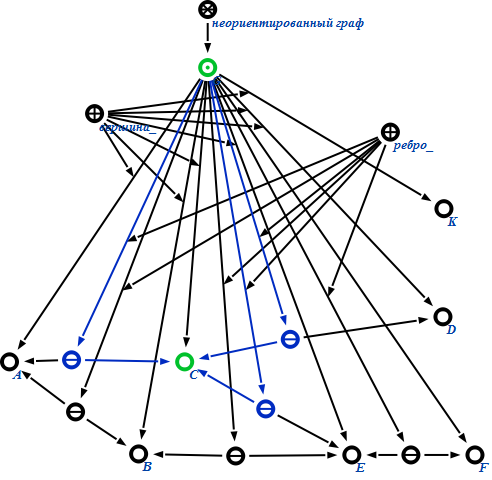
\includegraphics[scale=0.6]{4/libscprg/create_wave_search_edges}
  \caption{Поиск в указаном неориентированном граф инцидентных указанной вершине ребер}
  \label{fig:create_wave_search_edges}
\end{figure}

Теперь в новую волну \lstinline|new_wave| необходимо добавить ту
вершину \lstinline|other_vertex|, которая входит в
\lstinline|not_checked_vertexes|, и исключить ее из
\lstinline|not_checked_vertexes|. Эти действия продемонстрированы в
листинге ниже:
\begin{lstlisting}[texcl]
sc_addr create_wave(sc_session *s, sc_segment *seg, sc_addr graph,
    sc_addr wave, sc_addr not_checked_vertexes)
{
    // $\dots$

    sc_for_each (it_vertex) {
        // $\dots$

        sc_for_each (it_edge) {
            sc_addr edge = it_edge->value(2); // ребро, инцидентное  \verb|vertex|
            sc_addr other_vertex = get_other_vertex_incidence_edge(
                s, edge, vertex); // вершина, смежная \verb|vertex| и инцидентная \verb|edge|

            // Исключим вершину \verb|other_vertex| из множества непроверенных вершин и
            // включим в создаваемую волну.
            if (sc_set::exclude_from(s, other_vertex, not_checked_vertexes))
                sc_set::include_in(s, other_vertex, new_wave);
        }
    }

    return new_wave;
}
\end{lstlisting}

На этом написание функции \lstinline|create_wave| закончено, поэтому
вернемся к месту в цикле формирования списка волн, на котором мы
остановились. Новая волна создана, но она может быть пустой. Это
значит, что пути между вершинами не существует. Если волна пустая, то
необходимо выйти из функции \lstinline|find_min_path|:
\begin{lstlisting}[texcl]
sc_addr find_min_path(sc_session *s, sc_segment *seg, sc_addr graph,
    sc_addr beg_vertex, sc_addr end_vertex)
{
    // $\dots$

    // 3. Сформируем список волн.
    do {
        // $\dots$

        // Если новая волна пуста, то значит между вершинами не существует пути.
        if (sc_set::is_empty(s, new_wave)) {
            // Очищаем память и завершаем алгоритм.
            erase_waves_list(s, waves_list_head);
            s->erase_el(new_wave);
            s->erase_el(not_checked_vertexes);
            return 0;
        }

        // $\dots$
    } while (!sc_set::is_in(s, end_vertex, new_wave));

    // $\dots$
}
\end{lstlisting}

Обратите внимание, что при выходе из функции удалили все созданные
sc-конструкции. Функция \lstinline|erase_waves_list| имеет следующее
объявление (эту функцию вы рассмотрите самостоятельно):
\begin{lstlisting}[texcl]
/// Удаляет все волны из списка и список волн, начиная
/// с элемента списка @p \verb|waves_list_head|.
void erase_waves_list(sc_session *s, sc_addr waves_list_head);
\end{lstlisting}

Новая волна создана и непуста, значит пришла пора добавить ее в конец
списка волн:
\begin{lstlisting}[texcl]
sc_addr find_min_path(sc_session *s, sc_segment *seg, sc_addr graph,
    sc_addr beg_vertex, sc_addr end_vertex)
{
    // $\dots$

    // 3. Сформируем список волн.
    do {
        // $\dots$

        // Добавим новую волну в конец списка.
        sc_addr waves_list_curr = sc_list::create(s, seg, new_wave);
        sc_list::set_next(s, waves_list_tail, waves_list_curr);

        waves_list_tail = waves_list_curr;

        // Если в новой волне есть конечная вершина, то перейдем в начало цикла.
    } while (!sc_set::is_in(s, end_vertex, new_wave));

    // $\dots$
}
\end{lstlisting}

После цикла не забудем удалить уже ненужные sc-конструкции:
\begin{lstlisting}[texcl]
sc_addr find_min_path(sc_session *s, sc_segment *seg, sc_addr graph,
    sc_addr beg_vertex, sc_addr end_vertex)
{
    // $\dots$

    // Подчистим память.
    s->erase_el(not_checked_vertexes);

    // $\dots$
}
\end{lstlisting}

Итак\dots Мы закончили цикл формирования списка волн и переходим к
построению маршрута.

\subsubsection{Подготовка к формированию структуры маршрута}
\label{sec:libscprg_fmp_before_build_route}

Прежде, чем формировать структуру маршрута, нам необходимо создать
связку отношения \idtf{простая цепь*}. Это соотвествует шагу алгоритма
на странице \pageref{astep:S8_Create_route_tuple}.

Сгенерируем в sc-памяти связку отношения \idtf{простая цепь*}:
\begin{lstlisting}[texcl]
sc_addr find_min_path(sc_session *s, sc_segment *seg, sc_addr graph,
    sc_addr beg_vertex, sc_addr end_vertex)
{
    // $\dots$

    // 4. Создадим связку отношения \idtfm{простая цепь*}.
    sc_addr route = s->create_el(seg, SC_N_CONST); // связка отношения
    sc_set::include_in(s, route, graph_theory::simple_trail);

    // $\dots$
}
\end{lstlisting}

\emph{Обратите внимание}, что в листинге выше для включения связки в
отношение используется метод \lstinline|sc_set::include_in|, потому
что необходима генерация дуги в сегменте связки \lstinline|route|, а
не ключевого узла \lstinline|graph_theory::simple_trail|.

Теперь создадим компоненты связки \lstinline|route|:
\begin{lstlisting}[texcl]
sc_addr find_min_path(sc_session *s, sc_segment *seg, sc_addr graph,
    sc_addr beg_vertex, sc_addr end_vertex)
{
    // $\dots$

    // 5. Создадим компоненты связки \verb|route|.
    
    // Ориентированный граф структуры маршрута
    sc_addr route_struct = s->create_el(seg, SC_N_CONST);
    sc_set::include_in(s, route_struct, graph_theory::directed_graph);
    
    // Бинарное отношение посещения
    sc_addr route_visit = s->create_el(seg, SC_N_CONST);

    // $\dots$
}
\end{lstlisting}

Созданные компоненты включим в связку \lstinline|route|:
\begin{lstlisting}[texcl]
sc_addr find_min_path(sc_session *s, sc_segment *seg, sc_addr graph,
    sc_addr beg_vertex, sc_addr end_vertex)
{
    // $\dots$

    // 6. Добавим все компоненты в связку \verb|route|.
    sc_tup::add(s, route, N1_, route_struct);
    sc_tup::add(s, route, N2_, graph);
    sc_tup::add(s, route, N3_, route_visit);

    // $\dots$
}
\end{lstlisting}

В соответствии со следующим шагом алгоритма
(см. стр.~\pageref{S9_Add_end_vertex_visit_to_route_tuple}), добавим
посещение конечной вершины пути в структуру маршрута:
\begin{lstlisting}[texcl]
sc_addr find_min_path(sc_session *s, sc_segment *seg, sc_addr graph,
    sc_addr beg_vertex, sc_addr end_vertex)
{
    // $\dots$

    // 7. Добавим в простую цепь посещение конечной вершины.
    sc_addr end_vertex_visit = add_vertex_visit_to_route(s, route, end_vertex);

    // $\dots$
}
\end{lstlisting}

Функцию \lstinline|add_vertex_visit_to_route| объявим вот так:
\begin{lstlisting}[texcl]
/// Создает в структуре маршрута @p \verb|route| посещение вершины @p \verb|vertex|
/// и возвращает это посещение.
///
/// @note Все элементы генерируются в сегменте связки @p \verb|route|.
sc_addr add_vertex_visit_to_route(sc_session *s, sc_addr route, sc_addr vertex);
\end{lstlisting}

Прежде, чем рассматривать код этой функции, напишем две простые
вспомогательные функции для работы с маршрутом:
\begin{lstlisting}[texcl]
/// Возвращает структуру маршрута для связки отношения \idtfm{маршрут*}.
/// @note Структура маршрута - это компонент с атрибутом \idtfm{1\_}.
inline sc_addr get_route_struct(sc_session *s, sc_addr route)
{
    return sc_tup::at(s, route, N1_);
}

/// Возвращает отношение посещения для связки отношения \idtfm{маршрут*}.
/// @note Отношение посещения - это компонент с атрибутом \idtfm{3\_}.
inline sc_addr get_route_visit(sc_session *s, sc_addr route)
{
    return sc_tup::at(s, route, N3_);
}
\end{lstlisting}

Теперь перейдем к \lstinline|add_vertex_visit_to_route|. В начале
каждой функции для работы с маршрутом мы будем выполнять одно и то же
действие, а именно:
\begin{lstlisting}[texcl]
sc_addr add_vertex_visit_to_route(sc_session *s, sc_addr route, sc_addr vertex)
{
    // 1. Получим компоненты машрута: структуру маршрута и отношение посещения.
    sc_addr route_struct = get_route_struct(s, route); // структура маршрута
    sc_addr route_visit  = get_route_visit(s, route);  // отношение посещения

    // $\dots$
}
\end{lstlisting}

Зная структуру маршрута и отношение посещения, можно создать посещение
вершины в ориентированном графе структуры маршрута:
\begin{lstlisting}[texcl]
sc_addr add_vertex_visit_to_route(sc_session *s, sc_addr route, sc_addr vertex)
{
    // $\dots$

    // 2. Создадим посещение вершины.
    sc_addr vertex_visit = s->create_el(route->seg, SC_N_CONST);
    sc_tup::add(s, route->seg, route_struct, graph_theory::vertex_, vertex_visit);
    sc_rel::add_ord_tuple(s, route_visit, vertex_visit, vertex);

    return vertex_visit;
}
\end{lstlisting}

Теперь нам нужно пройтись по списку волн от конца в начало и построить найденный путь, что соответствует шагам алгоритма 

\subsection{Вывод маршрута на консоль}
\label{sec:libscprg_fmp_print_route}



%%% Local Variables: 
%%% mode: latex
%%% TeX-master: "main"
%%% End: 

